\documentclass[12pt,a4paper]{article}
\usepackage{geometry}
\geometry{left=2.5cm,right=2.5cm,top=2.0cm,bottom=2.5cm}
\usepackage[english]{babel}
\usepackage{amsmath,amsthm}
\usepackage{amsfonts}
\usepackage[longend,ruled,linesnumbered]{algorithm2e}
\usepackage{fancyhdr}
\usepackage{ctex}
\usepackage{array}
\usepackage{listings}
\usepackage{color}
\usepackage{graphicx}
\usepackage{tikz}

\begin{document}


\title{
{《优化理论与算法》第 3 次作业
}

}
\date{}

\author{
姓名：\underline{焦传斌}~~~~~~
学号：\underline{2024111223}~~~~~~}

\maketitle

\begin{itemize}
	\item 作业截止于{\bf 周五（3/27/2026）}，在Canvas系统中提交PDF或照片文件
	\item 作业题目的tex文件可以在Canvas中下载
	\item 鼓励相互讨论，但不要抄袭.
\end{itemize}
%%%%%%%%%%%%%%%%%%%%%%%%%%%%%%%%%%%%%%%%%%%%%%%%%%%%%%%%%%%%%%%%%
%%%%%%%%%%%%%%%%%%%%%%%%%%%%%%%%%%%%%%%%%%%%%%%%%%%%%%%%%%%%%%%%%

\section{阅读与积累}
\paragraph{1.1}
\begin{itemize}
	\item 阅读Bertsimas and Tsitsikils，也就是Introduction to Linear Optimization教材，第二章与第3.1,3.2节相关内容。
\end{itemize}

\section{习题}


\paragraph{2.1}
考虑如下线性规划标准型
\begin{equation*}
\begin{array}{lllll@{}ll}
\text{minimize}  & c^Tx\\
\text{subject to}&Ax=b \\
&x \geq 0
\end{array}
\end{equation*}

给定如下$A$和$b$的形式:
\[ A= \left[\begin{array}{c c c c c}
1 & 1& -1 & 2 & 1 \\4 & 2 & -2 &1 & 3 \\ 0 & 2 & 3 &-3 &1
\end{array}\right], b= \left[\begin{array}{c }
4  \\12 \\ 4
\end{array}\right] \]
\begin{enumerate}
    \item 下列哪组解是基本可行解? 
\[ x^{(1)}= \left[\begin{array}{c } 2  \\2 \\ 0 \\0 \\0 \end{array}\right],
x^{(2)}=\left[\begin{array}{c } 6  \\0 \\ 4 \\2 \\-2 \end{array}\right] ,
x^{(3)}=\left[\begin{array}{c } 0  \\0 \\ 0 \\0 \\4 \end{array}\right] ,
x^{(4)}=   \left[\begin{array}{c } 1  \\1 \\ 0 \\0 \\2 \end{array}\right],
x^{(5)}=   \left[\begin{array}{c } 0  \\4 \\ -\frac{8}{3} \\-\frac{4}{3} \\0 \end{array}\right]  \]
\item 找出所有的基本解和基本可行解
\end{enumerate}

\textbf{解：}

\textbf{(1) }

基本可行解需要满足：
\begin{itemize}
    \item 满足约束条件 $Ax = b$
    \item 满足非负性 $x \geq 0$
    \item 至多有 $m=3$ 个非零分量（基变量）
\end{itemize}



\textbf{$x^{(1)} = [2, 2, 0, 0, 0]^T$：}


\[
\left[\begin{array}{ccccc}
1 & 1 & -1 & 2 & 1 \\
4 & 2 & -2 & 1 & 3 \\
0 & 2 & 3 & -3 & 1
\end{array}\right]
\left[\begin{array}{c}
2 \\ 2 \\ 0 \\ 0 \\ 0
\end{array}\right]
=
\left[\begin{array}{c}
4 \\ 12 \\ 4
\end{array}\right] = b \quad \checkmark
\]

非零分量为2个（$x_1, x_2$），满足 $\leq m=3$，且 $x^{(1)} \geq 0$。基矩阵为 $B = [A_1, A_2]$，线性无关。


\textbf{$x^{(1)}$ 是基本可行解。}

\textbf{$x^{(2)} = [6, 0, 4, 2, -2]^T$：}

$x_5 = -2 < 0$，不满足非负性条件。

\textbf{$x^{(2)}$ 不是基本可行解。}

\textbf{$x^{(3)} = [0, 0, 0, 0, 4]^T$：}


\[
\left[\begin{array}{ccccc}
1 & 1 & -1 & 2 & 1 \\
4 & 2 & -2 & 1 & 3 \\
0 & 2 & 3 & -3 & 1
\end{array}\right]
\left[\begin{array}{c}
0 \\ 0 \\ 0 \\ 0 \\ 4
\end{array}\right]
=
\left[\begin{array}{c}
4 \\ 12 \\ 4
\end{array}\right] = b \quad \checkmark
\]

非零分量为1个（$x_5$），满足 $\leq m=3$，且 $x^{(3)} \geq 0$。

\textbf{$x^{(3)}$ 是基本可行解。}

\textbf{$x^{(4)} = [1, 1, 0, 0, 2]^T$：}


\[
\left[\begin{array}{ccccc}
1 & 1 & -1 & 2 & 1 \\
4 & 2 & -2 & 1 & 3 \\
0 & 2 & 3 & -3 & 1
\end{array}\right]
\left[\begin{array}{c}
1 \\ 1 \\ 0 \\ 0 \\ 2
\end{array}\right]
=
\left[\begin{array}{c}
4 \\ 12 \\ 4
\end{array}\right] = b \quad \checkmark
\]

非零分量为3个（$x_1, x_2, x_5$），恰好等于 $m=3$，且 $x^{(4)} \geq 0$。基矩阵为 $B = [A_1, A_2, A_5]$：

$\det\left[\begin{array}{ccc} 1 & 1 & 1 \\ 4 & 2 & 3 \\ 0 & 2 & 1 \end{array}\right]  = 0$

基矩阵奇异，列向量线性相关。

\textbf{$x^{(4)}$ 不是基本可行解。}

\textbf{$x^{(5)} = [0, 4, -\frac{8}{3}, -\frac{4}{3}, 0]^T$：}

$x_3 = -\frac{8}{3} < 0$ 且 $x_4 = -\frac{4}{3} < 0$，不满足非负性条件。

\textbf{$x^{(5)}$ 不是基本可行解。}

\textbf{答：$x^{(1)}$ 和 $x^{(3)}$ 是基本可行解。}

\textbf{(2) }

从5个变量中选择3个作为基变量，共有 $\binom{5}{3} = 10$ 种可能的基。

对每个基 $B$，求解 $Bx_B = b$，得到基解，然后检验非负性。

\textbf{基 $\{1,2,3\}$：} $B = \left[\begin{array}{ccc} 1 & 1 & -1 \\ 4 & 2 & -2 \\ 0 & 2 & 3 \end{array}\right]$，$\det(B) = -2 \neq 0$

$x_B = B^{-1}b = [4, -2, 2]^T$，$x = [4, -2, 2, 0, 0]^T$。$x_2 < 0$，不可行。

\textbf{基 $\{1,2,4\}$：} $B = \left[\begin{array}{ccc} 1 & 1 & 2 \\ 4 & 2 & 1 \\ 0 & 2 & -3 \end{array}\right]$，$\det(B) = -14 \neq 0$

$x_B = B^{-1}b = [3, -1, 1]^T$，$x = [3, -1, 0, 1, 0]^T$。$x_2 < 0$，不可行。

\textbf{基 $\{1,2,5\}$：} $B = \left[\begin{array}{ccc} 1 & 1 & 1 \\ 4 & 2 & 3 \\ 0 & 2 & 1 \end{array}\right]$，$\det(B) = 0$，奇异矩阵，无基解。

\textbf{基 $\{1,3,4\}$：} $B = \left[\begin{array}{ccc} 1 & -1 & 2 \\ 4 & -2 & 1 \\ 0 & 3 & -3 \end{array}\right]$，$\det(B) = 6 \neq 0$

$x_B = B^{-1}b = [2, 0, 1]^T$，$x = [2, 0, 0, 1, 0]^T$。$x \geq 0$，\textbf{基本可行解}。

\textbf{基 $\{1,3,5\}$：} $B = \left[\begin{array}{ccc} 1 & -1 & 1 \\ 4 & -2 & 3 \\ 0 & 3 & 1 \end{array}\right]$，$\det(B) = 10 \neq 0$

$x_B = B^{-1}b = [3, -1, 0]^T$，$x = [3, -1, 0, 0, 0]^T$。$x_3 < 0$，不可行。

\textbf{基 $\{1,4,5\}$：} $B = \left[\begin{array}{ccc} 1 & 2 & 1 \\ 4 & 1 & 3 \\ 0 & -3 & 1 \end{array}\right]$，$\det(B) = 14 \neq 0$

$x_B = B^{-1}b = [2, 0, 2]^T$，$x = [2, 0, 0, 0, 2]^T$。$x \geq 0$，\textbf{基本可行解}。

\textbf{基 $\{2,3,4\}$：} $B = \left[\begin{array}{ccc} 1 & -1 & 2 \\ 2 & -2 & 1 \\ 2 & 3 & -3 \end{array}\right]$，$\det(B) = -14 \neq 0$

$x_B = B^{-1}b = [2, 0, 1]^T$，$x = [0, 2, 0, 1, 0]^T$。$x \geq 0$，\textbf{基本可行解}。

\textbf{基 $\{2,3,5\}$：} $B = \left[\begin{array}{ccc} 1 & -1 & 1 \\ 2 & -2 & 3 \\ 2 & 3 & 1 \end{array}\right]$，$\det(B) = 10 \neq 0$

$x_B = B^{-1}b = [3, -1, 0]^T$，$x = [0, 3, -1, 0, 0]^T$。$x_3 < 0$，不可行。

\textbf{基 $\{2,4,5\}$：} $B = \left[\begin{array}{ccc} 1 & 2 & 1 \\ 2 & 1 & 3 \\ 2 & -3 & 1 \end{array}\right]$，$\det(B) = 14 \neq 0$

$x_B = B^{-1}b = [2, 0, 2]^T$，$x = [0, 2, 0, 0, 2]^T$。$x \geq 0$，\textbf{基本可行解}。即 $x^{(1)}$。

\textbf{基 $\{3,4,5\}$：} $B = \left[\begin{array}{ccc} -1 & 2 & 1 \\ -2 & 1 & 3 \\ 3 & -3 & 1 \end{array}\right]$，$\det(B) = 10 \neq 0$

$x_B = B^{-1}b = [0, 0, 4]^T$，$x = [0, 0, 0, 0, 4]^T$。$x \geq 0$，\textbf{基本可行解}。即 $x^{(3)}$。

\textbf{总结：}

所有基本解：
\begin{itemize}
    \item $[4, -2, 2, 0, 0]^T$
    \item $[3, -1, 0, 1, 0]^T$
    \item $[2, 0, 0, 1, 0]^T$
    \item $[3, -1, 0, 0, 0]^T$
    \item $[2, 0, 0, 0, 2]^T$
    \item $[0, 2, 0, 1, 0]^T$
    \item $[0, 3, -1, 0, 0]^T$
    \item $[0, 2, 0, 0, 2]^T$
    \item $[0, 0, 0, 0, 4]^T$
\end{itemize}

所有基本可行解：
\begin{itemize}
    \item $x = [2, 0, 0, 1, 0]^T$
    \item $x = [2, 0, 0, 0, 2]^T$
    \item $x = [0, 2, 0, 1, 0]^T$
    \item $x = [0, 2, 0, 0, 2]^T$
    \item $x = [0, 0, 0, 0, 4]^T$
\end{itemize}

\paragraph{2.2}
Bertsimas and Tsitsikils书中第一章课后题2.10.\textbf{问题描述} 考虑标准形式的多面体：
\[
P = \{ x \mid Ax = b, x \geq 0 \}。
\]
假设矩阵 \( A \) 的维度为 \( m \times n \)，且其行向量是线性无关的。对于以下每个陈述，判断其真伪。如果陈述为真，请给出证明；如果陈述为假，请提供一个反例。

\begin{enumerate}
    \item[(a)] 若 \( n = m + 1 \)，则 \( P \) 至多有两个基本可行解。
    \item[(b)] 在每个最优解处，至多有 \( m \) 个变量可以取正值。
    \item[(c)] 如果存在多个最优解，则至少存在两个基本可行解是最优的。
\end{enumerate}

\textbf{解：}

\textbf{(a) 若 $n = m + 1$，则 $P$ 至多有两个基本可行解。}

\textbf{答：真}

\textbf{证明：}

设 $A \in \mathbb{R}^{m \times n}$，$\operatorname{rank}(A) = m$，且 $n = m + 1$。

因为 $\operatorname{rank}(A) = m < n$，方程组 $Ax = b$ 的解空间维数为 $n - m = 1$。

设 $x^{(0)}$ 是 $Ax = b$ 的一个特解，$d \neq 0$ 是齐次方程 $Ad = 0$ 的一个非零解。则 $Ax = b$ 的通解为：
\[
x = x^{(0)} + td, \quad t \in \mathbb{R}
\]

加入非负约束 $x \geq 0$，即 $x^{(0)} + td \geq 0$，对每个分量 $i = 1, \ldots, n$：
\[
x^{(0)}_i + td_i \geq 0
\]

这给出 $t$ 的约束：
\begin{itemize}
    \item 若 $d_i > 0$：$t \geq -\frac{x^{(0)}_i}{d_i}$
    \item 若 $d_i < 0$：$t \leq -\frac{x^{(0)}_i}{d_i}$
\end{itemize}

因此可行的 $t$ 值构成一个区间 $[\alpha, \beta]$（可能无界或退化为单点）。

可行域 $P = \{x^{(0)} + td \mid t \in [\alpha, \beta]\}$ 是一条线段、射线或单点。

基本可行解对应于 $P$ 的极点。一条线段最多有2个端点，射线有1个端点，单点只有1个极点。

因此 $P$ 至多有2个基本可行解。

证毕。

\textbf{(b) 在每个最优解处，至多有 $m$ 个变量可以取正值。}

\textbf{答：假}

\textbf{反例：}

考虑线性规划：
\[
\min \quad x_1 + x_2 + x_3
\]
\[
\text{s.t.} \quad x_1 + x_2 + x_3 = 3, \quad x \geq 0
\]

这里 $m = 1$，$n = 3$，$A = [1, 1, 1]$，$b = [3]$。

其中一个最优解为 $x^* = [1, 1, 1]^T$，目标函数值为3。

在最优解 $x^* = [1, 1, 1]^T$ 处，有3个变量取正值，而 $3 > m = 1$。

因此陈述为假。

\textbf{(c) 如果存在多个最优解，则至少存在两个基本可行解是最优的。}

\textbf{答：真}

\textbf{证明：}

设线性规划问题为 $\min\{c^T x \mid Ax = b, x \geq 0\}$，可行域为 $P = \{x \mid Ax = b, x \geq 0\}$。

若存在多个最优解，则最优解集合 $F = \{x \in P \mid c^T x = z^*\}$ 是一个非单点的凸集（线性函数在凸集上的下水平集仍为凸集），因此 $F$ 至少包含一条线段。

由线性规划的标准结论：线性函数在多面体上的最小值一定在某个极点取得；若最优解不唯一，则最优解集合是一个面，其极点也都是最优解。

由于 $F$ 至少包含一条线段，而线段至少有两个端点（极点），因此 $F$ 至少包含两个极点。

在标准形下，极点 $\Leftrightarrow$ 基本可行解。

因此至少存在两个基本可行解是最优的。



\paragraph{2.3}
考虑以下问题

\begin{align*}
 \min \quad & -2x_1 - x_2 \\
\text{s.t} \quad & x_1 - x_2 \leq 2 \\
& x_1 + x_2 \leq 6 \\
& x_1, x_2 \geq 0.
\end{align*}


\begin{enumerate}
    \item[a)] 将问题转换为标准形式，并构造一个基本可行解，其中 \((x_1, x_2) = (0, 0)\)。
    \item[b)] 从(a)部分的基本可行解开始，执行单纯形法的完整表格实现。
    \item[c)] 绘制问题的图形表示，以原始变量 \(x_1, x_2\) 为基准，并指示单纯形算法所采取的路径。
\end{enumerate}

\textbf{解：}

\textbf{(a) 转换为标准形式}

引入松弛变量 $x_3, x_4 \geq 0$，将不等式约束转换为等式：

\begin{align*}
\min \quad & -2x_1 - x_2 \\
\text{s.t.} \quad & x_1 - x_2 + x_3 = 2 \\
& x_1 + x_2 + x_4 = 6 \\
& x_1, x_2, x_3, x_4 \geq 0
\end{align*}

当 $(x_1, x_2) = (0, 0)$ 时，从约束方程可得：
\[
x_3 = 2, \quad x_4 = 6
\]

因此基本可行解为：
\[
x = [0, 0, 2, 6]^T
\]

基变量为 $\{x_3, x_4\}$，非基变量为 $\{x_1, x_2\}$。

\textbf{(b) 单纯形法表格实现}

初始单纯形表（基 $B = \{3, 4\}$）：

\begin{table}[h]
\centering
\begin{tabular}{|c|cccc|c|}
\hline
B & -2 & -1 & 0 & 0 & 0 \\
\hline
3 & 1 & -1 & 1 & 0 & 2 \\
4 & 1 & 1 & 0 & 1 & 6 \\
\hline
\end{tabular}
\end{table}

检验数 $-2 < 0$，$-1 < 0$。选择 $x_1$ 入基。

最小比值检验：$\min\left\{\frac{2}{1}, \frac{6}{1}\right\} = 2$，$x_3$ 出基。


\begin{table}[h]
\centering
\begin{tabular}{|c|cccc|c|}
\hline
B & 0 & -3 & 2 & 0 & 4 \\
\hline
1 & 1 & -1 & 1 & 0 & 2 \\
4 & 0 & 2 & -1 & 1 & 4 \\
\hline
\end{tabular}
\end{table}

检验数 $-3 < 0$。选择 $x_2$ 入基。

最小比值检验：$\min\left\{\frac{4}{2}\right\} = 2$，$x_4$ 出基。



\begin{table}[h]
\centering
\begin{tabular}{|c|cccc|c|}
\hline
B & 0 & 0 & 1/2 & 3/2 & 10 \\
\hline
1 & 1 & 0 & 1/2 & 1/2 & 4 \\
2 & 0 & 1 & -1/2 & 1/2 & 2 \\
\hline
\end{tabular}
\end{table}

所有检验数 $\geq 0$，达到最优。

\textbf{最优解：}
\[
x_1^* = 4, \quad x_2^* = 2, \quad x_3^* = 0, \quad x_4^* = 0
\]

\textbf{最优目标函数值：}
\[
z^* = -2(4) - 2 = -10
\]

\textbf{(c) 图形表示}

可行域：
\begin{itemize}
    \item $x_1 - x_2 \leq 2$
    \item $x_1 + x_2 \leq 6$
    \item $x_1 \geq 0, x_2 \geq 0$
\end{itemize}

顶点：
\begin{itemize}
    \item $A = (0, 0)$：初始基本可行解
    \item $B = (2, 0)$：$x_1 - x_2 = 2$ 与 $x_2 = 0$ 的交点
    \item $C = (4, 2)$：$x_1 - x_2 = 2$ 与 $x_1 + x_2 = 6$ 的交点（最优解）
    \item $D = (0, 6)$：$x_1 = 0$ 与 $x_1 + x_2 = 6$ 的交点
\end{itemize}

\begin{figure}[h]
\centering
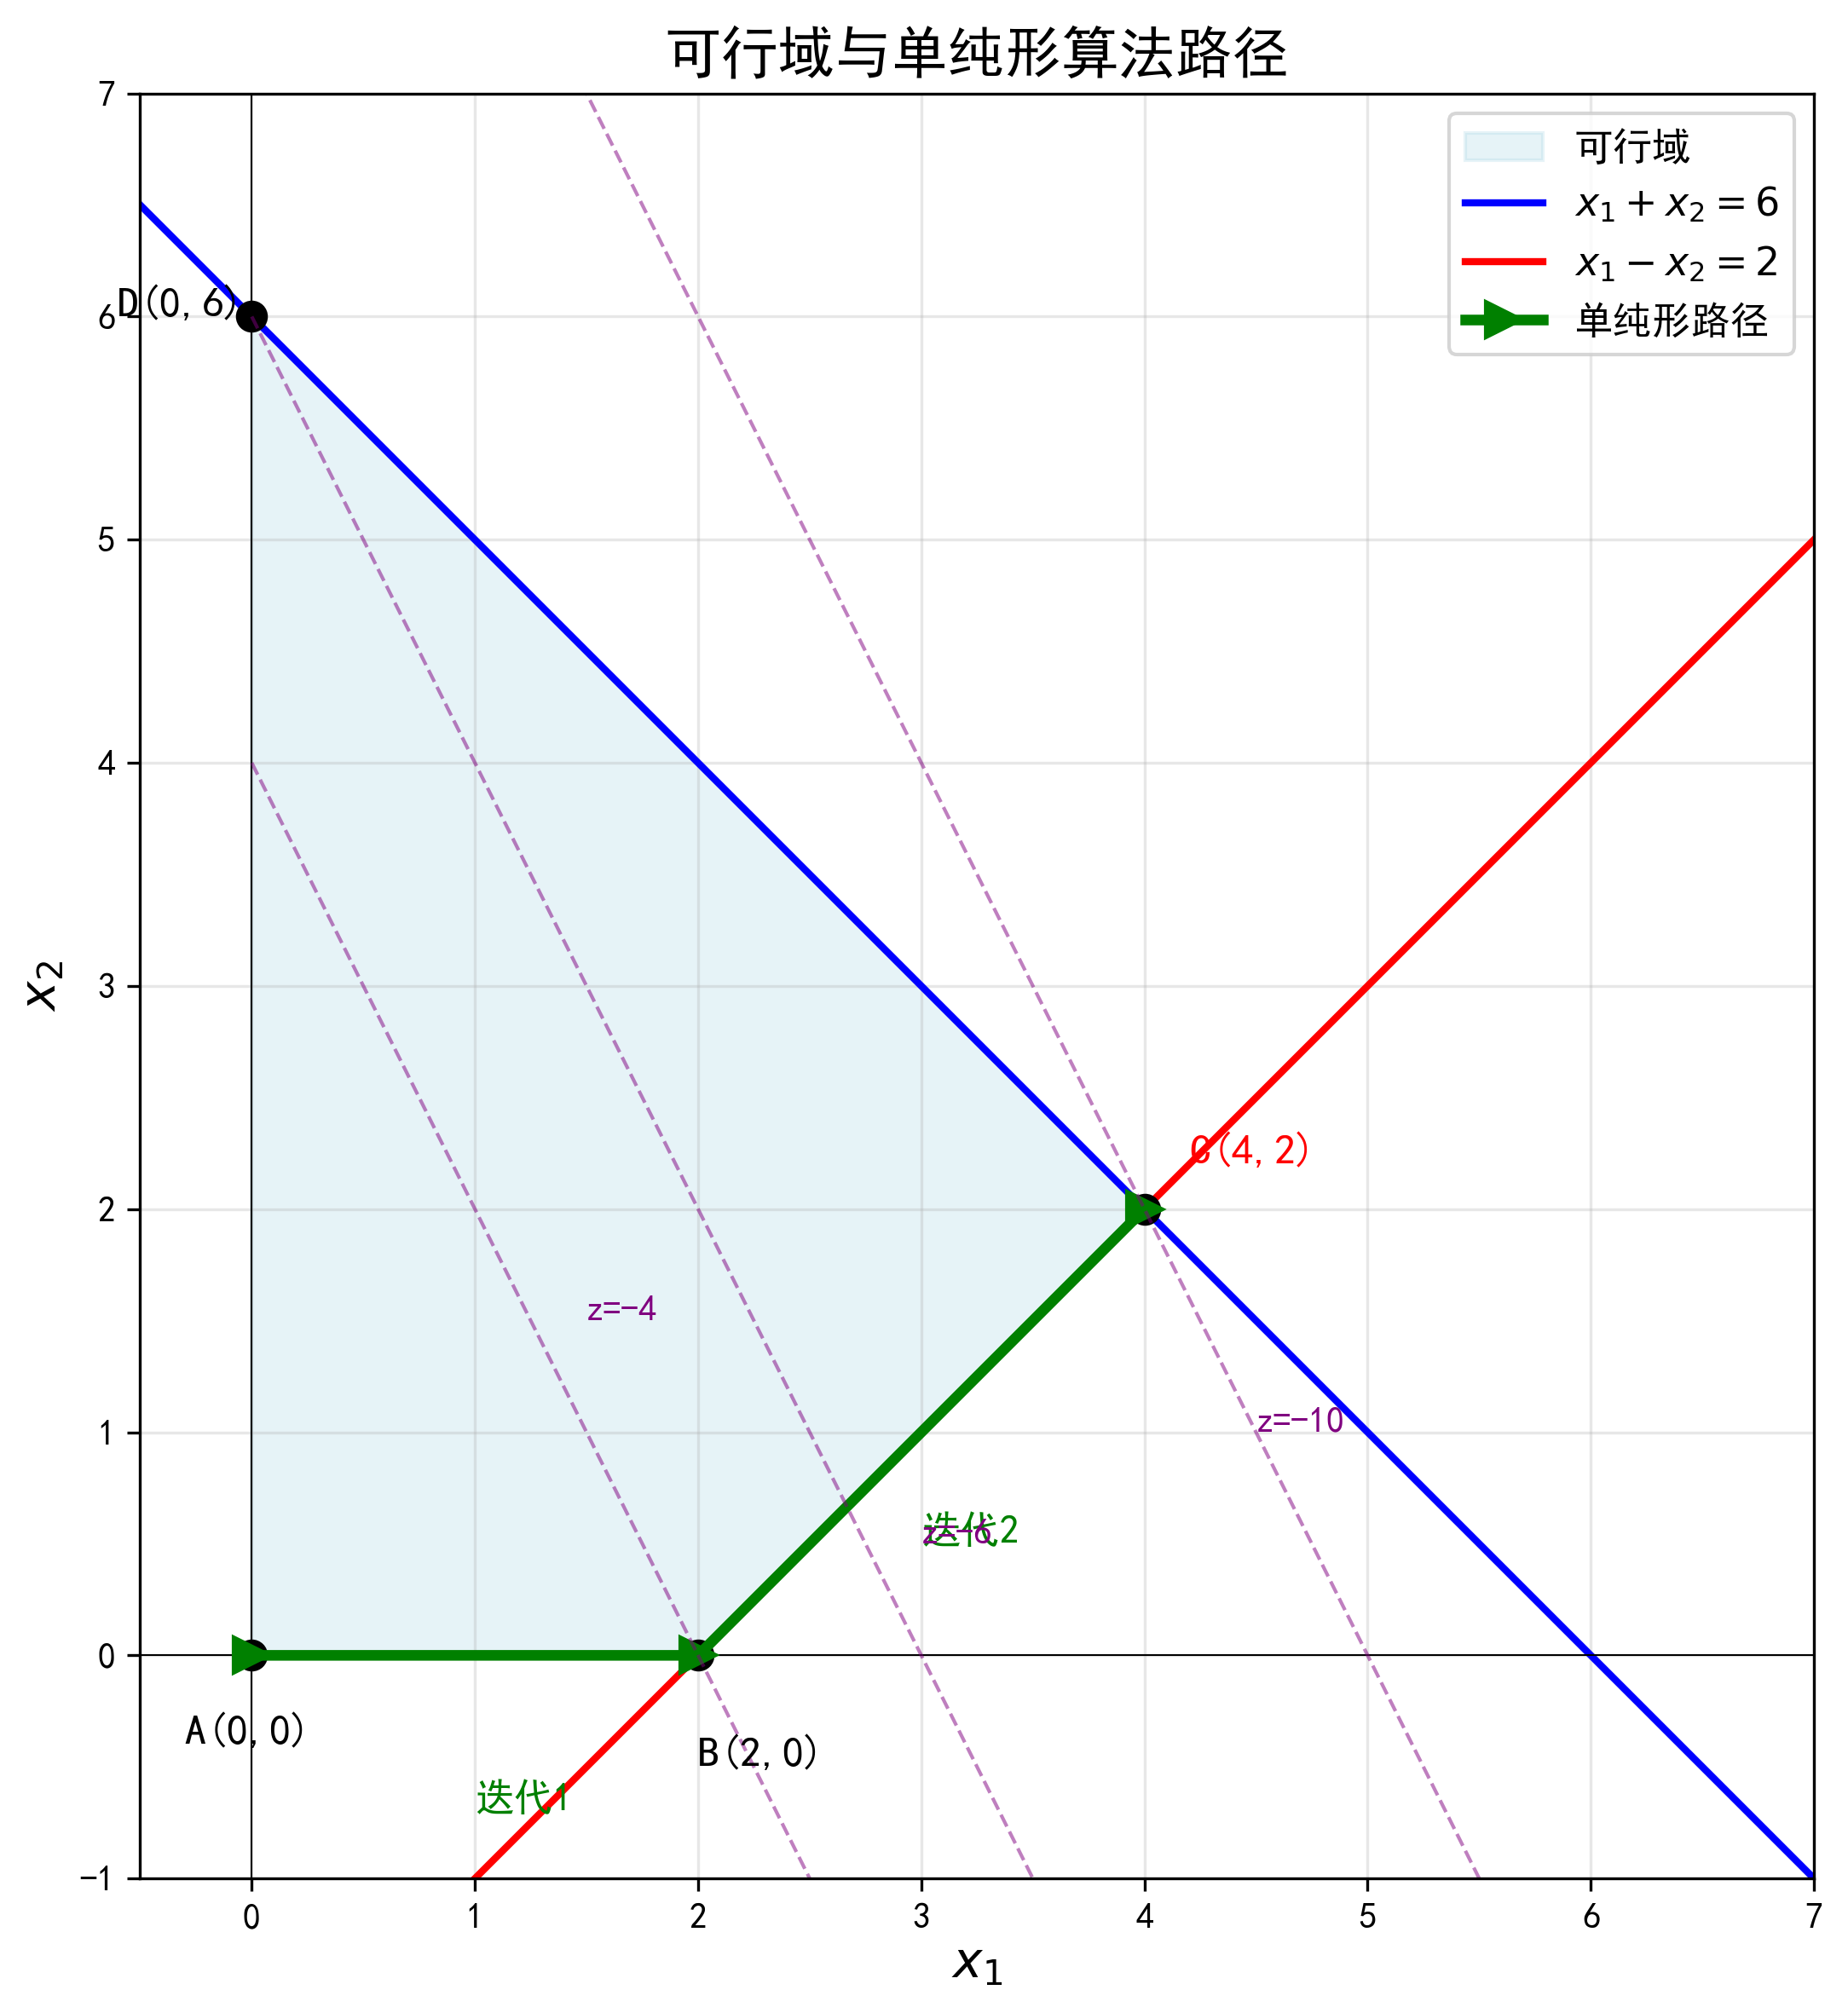
\includegraphics[width=0.7\textwidth]{simplex_path.png}
\caption{可行域与单纯形算法路径}
\end{figure}

\textbf{单纯形算法路径：}
\[
A(0, 0) \xrightarrow{x_1 \text{入基}} B(2, 0) \xrightarrow{x_2 \text{入基}} C(4, 2) \text{（最优）}
\]

单纯形法沿着可行域的边从一个顶点移动到相邻顶点，每次迭代目标函数值都在减小，直到达到最优解 $C(4,2)$，此时 $z^* = -10$。


\paragraph{2.4}
课件《单纯形法初窥》P31页所展示的线性规划，如果第一次迭代选$x_2$为入基变量，请展示后续迭代直至取到最优解。（后续迭代过程中若有多可行的入基或出基变量则序号较小的）

\textbf{解：}

题目的线性规划问题为：
\begin{align*}
\min \quad & -10x_1 - 12x_2 - 12x_3 \\
\text{s.t.} \quad & x_1 + 2x_2 + 2x_3 \leq 20 \\
& 2x_1 + x_2 + 2x_3 \leq 20 \\
& 2x_1 + 2x_2 + x_3 \leq 20 \\
& x_1, x_2, x_3 \geq 0
\end{align*}

引入松弛变量 $x_4, x_5, x_6$，初始基 $B = \{4, 5, 6\}$。

\textbf{初始单纯形表：}

\begin{table}[h]
\centering
\begin{tabular}{|c|cccccc|c|}
\hline
B & -10 & -12 & -12 & 0 & 0 & 0 & 0 \\
\hline
4 & 1 & 2 & 2 & 1 & 0 & 0 & 20 \\
5 & 2 & 1 & 2 & 0 & 1 & 0 & 20 \\
6 & 2 & 2 & 1 & 0 & 0 & 1 & 20 \\
\hline
\end{tabular}
\end{table}

检验数行：$-10, -12, -12$ 都小于0。题目要求选 $x_2$ 入基。

最小比值检验：$\min\left\{\frac{20}{2}, \frac{20}{1}, \frac{20}{2}\right\} = \min\{10, 20, 10\} = 10$

有两个相同的最小比值（第1行和第3行），选择序号较小的，即 $x_4$ 出基。




\begin{table}[h]
\centering
\begin{tabular}{|c|cccccc|c|}
\hline
B & -10 & 0 & -12 & 6 & 0 & 0 & -120 \\
\hline
2 & 1/2 & 1 & 1 & 1/2 & 0 & 0 & 10 \\
5 & 3/2 & 0 & 1 & -1/2 & 1 & 0 & 10 \\
6 & 1 & 0 & -1 & -1 & 0 & 1 & 0 \\
\hline
\end{tabular}
\end{table}

检验数：$-10 < 0$，$-12 < 0$。选择 $x_3$ 入基。

最小比值检验：$\min\left\{\frac{10}{1}, \frac{10}{1})\right\} = 10$

有两个相同的最小比值（第1行和第2行），选择序号较小的，即 $x_2$ 出基。



\begin{table}[h]
\centering
\begin{tabular}{|c|cccccc|c|}
\hline
B & -4 & 12 & 0 & 12 & 0 & 0 & -240 \\
\hline
3 & 1/2 & 1 & 1 & 1/2 & 0 & 0 & 10 \\
5 & 1 & -1 & 0 & -1 & 1 & 0 & 0 \\
6 & 3/2 & 1 & 0 & -1/2 & 0 & 1 & 10 \\
\hline
\end{tabular}
\end{table}

检验数：$-4 < 0$。选择 $x_1$ 入基。

最小比值检验：$\min\left\{\frac{10}{1/2}, \frac{0}{1}, \frac{10}{3/2}\right\} = \min\{20, 0, 6.67\} = 0$






\begin{table}[h]
\centering
\begin{tabular}{|c|cccccc|c|}
\hline
B & 0 & 8 & 0 & 8 & 4 & 0 & -240 \\
\hline
3 & 0 & 3/2 & 1 & 1 & -1/2 & 0 & 10 \\
1 & 1 & -1 & 0 & -1 & 1 & 0 & 0 \\
6 & 0 & 5/2 & 0 & 1 & -3/2 & 1 & 10 \\
\hline
\end{tabular}
\end{table}

所有检验数 $\geq 0$，达到最优。

\textbf{最优解：}$x_1 = 0, x_2 = 0, x_3 = 10$，最优目标函数值 $z^* = -240$。



\paragraph{2.5 (附加加分题)} 
\textbf{问题描述}

考虑全球货币市场。对于两种货币（例如日元和美元），它们之间存在一个汇率（例如，从表中可见，美元兑换日元的汇率约为 133.38）。一个无套利市场意味着不存在这样一种方法，使得通过一系列兑换（例如，美元兑换成日元，再兑换成欧元，然后兑换成英镑，最后回到美元）可以最终得到超过 1 美元的金额。

\textbf{外汇市场的实际交易数据（2002年2月14日）}

\begin{table}[ht]
	\caption{外汇市场中的汇率} 
	\centering 
	\begin{tabular}{c c c c c c} 
    \hline\hline
		从 & & 美元 & 欧元 & 英镑 & 日元\\ 
        \hline
		兑换为 & 美元 &        & 0.8706 & 1.4279 & 0.00750 \\ 
		兑换为 & 欧元 & 1.1486 &        & 1.6401 & 0.00861 \\
		兑换为 & 英镑 & 0.7003 & 0.6097 &        & 0.00525 \\
		兑换为 & 日元 & 133.38 & 116.12 & 190.45 &         \\ \hline\hline
	\end{tabular}
	\label{table:exchange} 
\end{table}

例如，1 美元兑换成欧元可得到 1.1486 欧元。从上表中看，套利机会并不明显，但如果没有任何转换成本，通过美元—英镑—日元—美元的路径，每兑换 1 美元可获得额外的 0.0003 美元，而如果按照美元—日元—欧元—美元的路径，每兑换 1 美元则损失约 0.0002 美元。

\textbf{如何识别套利机会？}

给定一个汇率表，如何构建一个线性规划模型来识别此类套利机会？

\textbf{提示}：可以将货币兑换看作图上的流或路径。例如，可以定义决策变量 \( x_{ij} \) 表示将货币 \( i \) 兑换为货币 \( j \) 的金额。

\textbf{解：}

\textbf{问题建模}

设有 $n$ 种货币，设起始货币为 $s$（如美元），设时期总数为 $T$。设 $r_{ij}$ 为从货币 $i$ 兑换为货币 $j$ 的汇率（即1单位货币 $i$ 可兑换 $r_{ij}$ 单位货币 $j$）。

\textbf{决策变量与状态变量：}

\begin{itemize}
    \item $x_{ij}^t \geq 0$：在时期 $t$ 从货币 $i$ 兑换为货币 $j$ 的金额（$t=0,\ldots,T-1$）
    \item $y_i^t \geq 0$：在时期 $t$ 末尾持有货币 $i$ 的金额（$t=0,\ldots,T$）
\end{itemize}

\textbf{初始条件：}

从1单位起始货币 $s$ 开始，其他货币初始为0：
\[
y_s^0 = 1, \quad y_i^0 = 0 \quad (i \neq s)
\]

\textbf{完整的线性规划模型：}

\begin{align*}
\max \quad & y_s^T \\
\text{s.t.} \quad & y_s^0 = 1, \quad y_i^0 = 0 \quad (i \neq s) \\
& \sum_{j \neq i} x_{ij}^t \leq y_i^t, \quad \forall i, t=0,\ldots,T-1 \\
& y_i^{t+1} = y_i^t - \sum_{j \neq i} x_{ij}^t + \sum_{j \neq i} r_{ji} x_{ji}^t, \quad \forall i, t=0,\ldots,T-1 \\
& x_{ij}^t \geq 0, \quad \forall i \neq j, t=0,\ldots,T-1 \\
& y_i^t \geq 0, \quad \forall i, t=0,\ldots,T
\end{align*}

\textbf{对于给定的4种货币问题的求解：}

设起始货币 $s = 1$（美元），货币编号：1=美元，2=欧元，3=英镑，4=日元。不妨取时期数 $T = 4$。

根据表格数据，汇率矩阵为：
\[
R = \begin{bmatrix}
- & 1.1486 & 0.7003 & 133.38 \\
0.8706 & - & 0.6097 & 116.12 \\
1.4279 & 1.6401 & - & 190.45 \\
0.00750 & 0.00861 & 0.00525 & -
\end{bmatrix}
\]

\textbf{使用COPT求解结果：}

最优目标函数值：$z^* = 1.00070$

\textbf{各时期货币持有量：}

\begin{table}[h]
\centering
\begin{tabular}{|c|c|c|c|c|c|}
\hline
时期 & 美元 & 欧元 & 英镑 & 日元 & 总计 \\
\hline
$t=0$ & 1.0000000000 & 0 & 0 & 0 & 1.0000 \\
$t=1$ & 0 & 0 & 0 & 133.3800000 & 133.38 \\
$t=2$ & 1.0003500000 & 0 & 0 & 0 & 1.00035 \\
$t=3$ & 0 & 0 & 0 & 133.4266830 & 133.4267 \\
$t=4$ & 1.0007001225 & 0 & 0 & 0 & 1.00070 \\
\hline
\end{tabular}
\end{table}









\[
1.0000 \text{ 美元} \xrightarrow[\text{时期0}]{\times 133.38} 133.38 \text{ 日元} \xrightarrow[\text{时期1}]{\times 0.00750} 1.00035 \text{ 美元}\]
\[
\xrightarrow[\text{时期2}]{\times 133.38} 133.4267 \text{ 日元} \xrightarrow[\text{时期3}]{\times 0.00750} 1.00070 \text{ 美元}
\]

    套利收益率：$ 0.070\%$





\textbf{本问题的结论：}

在给定的汇率数据下，当时期数 $T = 4$ 时，多时期模型的最优解为 $z^* = 1.00070$，套利收益率为 $0.070\%$。

\textbf{套利判断：}

如果最优目标函数值 $y_s^T > 1$，则存在套利机会；如果 $y_s^T = 1$，则市场无套利。在本问题中，$y_s^T = 1.00070 > 1$，确实存在套利机会。值得注意的是，当时期数 $T$ 增大时，套利收益也随之增大，这反映了可以重复套利循环的特点。

\vspace{0.5cm}

\textbf{进一步分析：不同初始货币的套利情况（}$T=4$\textbf{）}

使用COPT求解器分别以欧元、英镑和日元为初始货币进行求解，其结果汇总如下：

\begin{table}[h]
\centering
\caption{不同初始货币的套利结果对比}
\begin{tabular}{|c|c|c|c|}
\hline
初始货币 & 最优目标函数值 & 套利收益（绝对值） & 套利收益率 \\
\hline
美元 & 1.0007001225 & 0.0007001225 & 0.070012\% \\
欧元 & 1.0003211499 & 0.0003211499 & 0.032115\% \\
英镑 & 1.0003083554 & 0.0003083554 & 0.030836\% \\
日元 & 1.0007001225 & 0.0007001225 & 0.070012\% \\
\hline
\end{tabular}
\end{table}








    \textbf{最优套利路径不同}：
    \begin{itemize}
        \item 美元初始：美元 → 日元 → 美元（反复2次）
        \item 日元初始：日元 → 美元 → 日元（反复2次）
        \item 欧元初始：欧元 → 美元 → 日元 → 美元 → 欧元
        \item 英镑初始：英镑 → 美元 → 日元 → 美元 → 英镑
    \end{itemize}
    

\textbf{结论：}
发现美元，日元相互兑换有互相套利机会且较大，以欧元和英镑初始货币套利也主要依赖于美日元相互兑换。


\end{document}

